\section{Green's Theorem}\label{sec:greens}

We will now see a way of evaluating the line integral of a \emph{smooth} vector field around a simple closed curve. A vector field $\vecf(x,y) = P(x,y)\,\veci + Q(x,y)\,\vecj$ is \textbf{smooth} if its component functions $P(x,y)$ and $Q(x,y)$ are smooth.\index{vector field!smooth} We will use \emph{Green's Theorem} (sometimes called \emph{Green's Theorem in the plane}) to relate the \emph{line} integral around a closed curve with a \emph{double} integral over the region inside the curve:\index{Green's Theorem}

\theorem{thm:green}{Green's Theorem}{Let $R$ be a region in $\mathbb{R}^2$ whose boundary is a simple closed curve $C$ which is piecewise smooth. Let $\vecf(x,y) = P(x,y)\,\veci + Q(x,y)\,\vecj$ be a smooth vector field defined on both $R$ and $C$. Then
  \begin{equation}\label{eqn:green}
   \oint_{C}\vecf\cdot d\vecr
   = \iint_{R} \left( \frac{\partial Q}{\partial x} - \frac{\partial P}{\partial y} \right)\,dA ,
  \end{equation}
  where $C$ is traversed so that $R$ is always on the left side of $C$.}

\begin{proof}
 We will prove the theorem in the case for a \emph{simple} region $R$, that is, where the boundary curve $C$ can be written as $C = C_1 \cup C_2$ in two distinct ways:
 \begin{align}
  C_1 &= \text{the curve $y = y_1(x)$ from the point $X_1$ to the point $X_2$} \label{green_bottom}\\
  C_2 &= \text{the curve $y = y_2(x)$ from the point $X_2$ to the point $X_1$,}\label{green_top}
 \end{align}
 where $X_1$ and $X_2$ are the points on $C$ farthest to the left and right, respectively; and
 \begin{align}
  C_1 &= \text{the curve $x = x_1(y)$ from the point $Y_2$ to the point $Y_1$}\label{green_left}\\
  C_2 &= \text{the curve $x = x_2(y)$ from the point $Y_1$ to the point $Y_2$,}\label{green_right}
 \end{align}
 where $Y_1$ and $Y_2$ are the lowest and highest points, respectively, on $C$.
 See \autoref{fig_green_simple}.

 \begin{lxfigure}
 \centering
 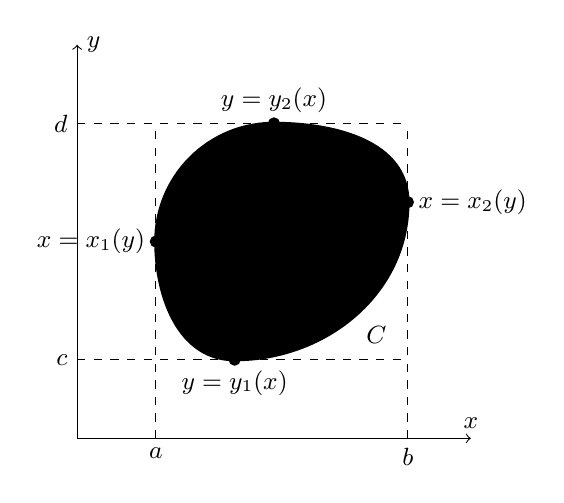
\begin{tikzpicture}
  \usetikzlibrary{arrows}
  \draw [black,->] (0,0) -- (5,0) node[above] {\small$x$};
  \draw [black,->] (0,0) -- node[right,pos=1]{\small$y$} (0,5);
  \filldraw [draw={\colorone},very thick,fill={\coloronefill}]
   (1,2.5)node[left]{\small $x = x_1(y)$}node[right]{\small $X_1$}
   to[out=90,in=180] node [sloped]{\large $\blacktriangleleft$}(2.5,4)
   node[below]{\small $Y_2$}node[above] {\small $y = y_2(x)$}
   to[out=0,in=90](4.2,3) node[right]{\small $x = x_2(y)$}node[left]{\small $X_2$}
   to[out=270,in=0] node [sloped]{\large $\blacktriangleright$}
   node[below right]{\small$C$}
   (2,1)node[above]{\small $Y_1$}node[below]{\small $y = y_1(x)$}
   to[out=180,in=270] cycle;
  \node at (2.5,2.5) {\small $R$};
  \draw [dashed] (1,0)node[below]{\small$a$} -- (1,4);
  \draw [dashed] (4.2,0)node[below]{\small$b$} -- (4.2,4);
  \draw [dashed] (0,4)node[left]{\small$d$} -- (4.2,4);
  \draw [dashed] (0,1)node[left]{\small$c$} -- (4.2,1);
  \fill[draw={\colorone},fill={\colorone}] (1,2.5) circle (2pt);
  \fill[draw={\colorone},fill={\colorone}] (2.5,4) circle (2pt);
  \fill[draw={\colorone},fill={\colorone}] (4.2,3) circle (2pt);
  \fill[draw={\colorone},fill={\colorone}] (2,1) circle (2pt);
 \end{tikzpicture}
 \caption{Figure for Green's Theorem on a simple region.}
 \label{fig_green_simple}
 \end{lxfigure}

 Integrate $P(x,y)$ around $C$ using the representation $C = C_1 \cup C_2$ given by Equations \eqref{green_bottom} and \eqref{green_top}. Since $y = y_1(x)$ along $C_1$ (as $x$ goes from $a$ to $b$) and $y = y_2(x)$ along $C_2$ (as $x$ goes from $b$ to $a$), as we see from \autoref{fig_green_simple}, then we have
 \begin{align*}
  \oint_C P(x,y)\,dx &= \int_{C_1} P(x,y)\,dx + \int_{C_2} P(x,y)\,dx\\
   &= \int_a^b P(x,y_1(x))\,dx + \int_b^a P(x,y_2(x))\,dx\\
   &= \int_a^b P(x,y_1(x))\,dx - \int_a^b P(x,y_2(x))\,dx\\[6pt]
   &= -\int_a^b \left( P(x,y_2(x)) - P(x,y_1(x)) \right)\,dx\\[6pt]
   &= -\int_a^b \left( P(x,y) \,\Big|_{y = y_1(x)}^{y = y_2(x)} \,\right)\,dx\\[6pt]
   &= -\int_a^b \int_{y_1(x)}^{y_2(x)} \frac{\partial P(x,y)}{\partial y}\,dy\,dx \text{ (by the Fundamental Theorem of Calculus)}\\[6pt]
   &= -\iint_{R} \frac{\partial P}{\partial y}\,dA .
 \end{align*}
 Likewise, integrate $Q(x,y)$ around $C$ using the representation $C = C_1 \cup C_2$ given by Equations \eqref{green_left} and \eqref{green_right}. Since $x = x_1(y)$ along $C_1$ (as $y$ goes from $d$ to $c$) and $x = x_2(y)$ along $C_2$ (as $y$ goes from $c$ to $d$), as we see from \autoref{fig_green_simple}, then we have
 \begin{align*}
  \oint_C Q(x,y)\,dy &= \int_{C_1} Q(x,y)\,dy + \int_{C_2} Q(x,y)\,dy\\
   &= \int_d^c Q(x_1(y),y)\,dy + \int_c^d Q(x_2(y),y)\,dy\\
   &= -\int_c^d Q(x_1(y),y)\,dy + \int_c^d Q(x_2(y),y)\,dy\\[6pt]
   &= \int_c^d \left( Q(x_2(y),y) - Q(x_1(y),y) \right)\,dy\\[6pt]
   &= \int_c^d \left( Q(x,y) \,\Big|_{x = x_1(y)}^{x = x_2(y)} \,\right)\,dy\\[6pt]
   &= \int_c^d \int_{x_1(y)}^{x_2(y)} \frac{\partial Q(x,y)}{\partial x}\,dx\,dy \text{ (by the Fundamental Theorem of Calculus)}\\[6pt]
   &= \iint_{R} \frac{\partial Q}{\partial x}\,dA .
 \end{align*}
Putting this together, we have
 \begin{align*}
  \oint_{C}\vecf\cdot d\vecr &= \oint_C P(x,y)\,dx + \oint_C Q(x,y)\,dy\\[6pt]
   &= -\iint_{R} \frac{\partial P}{\partial y}\,dA + \iint_{R} \frac{\partial Q}{\partial x}\,dA\\[6pt]
   &= \iint_{R} \left( \frac{\partial Q}{\partial x} - \frac{\partial P}{\partial y} \right)\,dA .\qedhere
 \end{align*}
\end{proof}

Though we proved Green's Theorem only for a simple region $R$, the theorem can also be proved for more general regions (say, a union of simple regions).% See \cite[\S\,15.31]{tm} for a discussion of some of the difficulties involved when the boundary curve is ``complicated''.

\youtubeVideo{a_zdFvYXX_c}{Green's Theorem}

\example{exmp_greenexmp}{Using Green's Theorem}{Evaluate $\oint_{C} (x^2 + y^2 )\,dx + 2xy\,dy$, where $C$ is the boundary (traversed counterclockwise) of the region
  $R = \{(x,y): 0 \le x \le 1,2x^2 \le y \le 2x \}$.}{%
 \mtable{Figure for \autoref{exmp_greenexmp}}{fig_greenexmp}{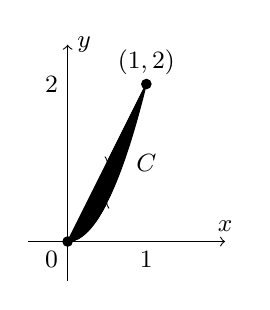
\begin{tikzpicture}
   \usetikzlibrary{arrows}
   \draw[draw={\colorone},fill={\coloronefill}](0,0)parabola(1,2)
    node[above]{\small$(1,2)$}--cycle;
   \draw [black,->] (-0.5,0) --node[above,pos=1,color=black]{\small$x$} (2,0);
   \draw [black,->] (0,-0.5) --node[right,pos=1,color=black]{\small$y$} (0,2.5);
   \node[below left]at(0,0){\small$0$};
   \draw [draw={\colorone},->] (0,0) parabola (0.5,0.5);
   \draw [draw={\colorone},->] (1,2) -- (0.5,1);
   \node [left] at (0,2) {\small $2$};
   \node [below] at (1,0) {\small $1$};
   \node at (1,1) {\small $C$};
   \fill[draw={\colorone},fill={\colorone}] (0,0) circle (1.7pt);
   \fill[draw={\colorone},fill={\colorone}] (1,2) circle (1.7pt);
  \end{tikzpicture}}
  %
 $R$ is the shaded region in \autoref{fig_greenexmp}. By Green's Theorem, for
 $P(x,y)=x^2 + y^2$ and $Q(x,y)=2xy$, we have
 \begin{align*}
  \oint_C (x^2 + y^2 )\,dx + 2xy\,dy &= \iint_{R} \left( \frac{\partial Q}{\partial x} -
   \frac{\partial P}{\partial y} \right)\,dA\\
   &= \iint_{R} (2y - 2y)\,dA
   = \iint_{R} 0\,dA = 0 .
 \end{align*}
 We actually already knew that the answer was zero. Recall from \autoref{exmp_lineintexmpclosed} in \autoref{sec:line_int_props} that the vector field $\vecf(x,y) = ( x^2 + y^2 )\,\veci + 2xy\,\vecj$ has a potential function $F(x,y)=\frac{1}{3}x^3 + xy^2$, and so $\oint_{C}\vecf\cdot d\vecr = 0$ by \autoref{cor:lineintsuffpath}.}

\example*{exmp_greenhole}{Green's Theorem with a Hole}{Let $\vecf(x,y) = P(x,y)\,\veci + Q(x,y)\,\vecj$, where
 \[
  P(x,y) = \frac{-y}{x^2 + y^2} \quad\text{and}\quad Q(x,y) = \frac{x}{x^2 + y^2} ,
 \]
 and let $R =\lbrace\,(x,y): 0 < x^2 + y^2 \le 1\,\rbrace$. For the boundary curve $C:x^2 + y^2 = 1$, traversed counterclockwise, it was shown in Exercise \ref{contra_green}(b) in \autoref{sec:line_int_props} that $\oint_{C}\vecf\cdot d\vecr = 2\pi$. But
 \[
  \frac{\partial Q}{\partial x} = \frac{y^2 - x^2}{(x^2 + y^2 )^2} = \frac{\partial P}{\partial y} 
  \Rightarrow 
  \iint_{R} \left( \frac{\partial Q}{\partial x} - \frac{\partial P}{\partial y} \right)\,dA =
  \iint_{R} 0 \,dA = 0.
 \]

This would seem to contradict Green's Theorem. However, note that $R$ is not the \emph{entire} region enclosed by $C$, since the point $(0,0)$ is not contained in $R$. That is, $R$ has a ``hole'' at the origin, so Green's Theorem does not apply.}

\mtable{The annulus $R$}{fig_annulus}{\begin{tikzpicture}[scale=2]
% \usetikzlibrary{arrows}
 \filldraw [draw={\colorone},fill={\coloronefill}] (0,0) circle (1);
 \filldraw [draw={\colorone},fill=white] (0,0) circle (0.5);
 \draw [black,->] (-1.2,0) --node[above,pos=1]{\small$x$} (1.2,0);
 \draw [black,->] (0,-1.2) --node[right,pos=1]{\small$y$} (0,1.2);
% \pgfputat{\pgfpointxyz{2.9}{0.2}{0}}{\pgfbox[center,center]{\small $x$}};
% \pgfputat{\pgfpointxyz{0.2}{2.9}{0}}{\pgfbox[center,center]{\small $y$}};
 \node[below right]at(0,0){\small$0$};
% \pgfputat{\pgfpointxyz{0.15}{-0.2}{0}}{\pgfbox[center,center]{\small $0$}};
 \node [above right] at (45:1) {\small $C_1$};
 \node [right] at (45:0.5) {\small $C_2$};
 \node [above left] at (0,1) {\small $1$};
 \node [below right] at (1,0) {\small $1$};
 \node [above left] at (0,0.5) {\small $\frac12$};
 \node [below right] at (0.5,0) {\small $\frac12$};
 \node at (.7:45) {\small $R$};
 \node [rotate=45] at (135:.5) {$\blacktriangleright$};
 \node [rotate=-45] at (45:1) {$\blacktriangleleft$};
\end{tikzpicture}}
If we modify the region $R$ to be the \emph{annulus} $R =\lbrace\,(x,y): 1/4 \le x^2 + y^2 \le 1\,\rbrace$ (see \autoref{fig_annulus}), and take the ``boundary'' $C$ of $R$ to be $C = C_1 \cup C_2$, where $C_1$ is\index{annulus} the unit circle $x^2 + y^2 = 1$ traversed counterclockwise and $C_2$ is the circle $x^2 + y^2 = 1/4$ traversed \emph{clockwise}, then it can be shown (see Exercise \ref{const_closed_int}) that
\[\oint_{C}\vecf\cdot d\vecr = 0 .\]
We would still have $\iint_{R} \left( \frac{\partial Q}{\partial x} - \frac{\partial P}{\partial y} \right)\,dA= 0$, so for this $R$ we would have
\[
 \oint_{C}\vecf\cdot d\vecr =
 \iint_{R} \left( \frac{\partial Q}{\partial x} - \frac{\partial P}{\partial y} \right)\,dA ,
\]
which shows that Green's Theorem holds for the annular region $R$.\bigskip

It turns out that Green's Theorem can be extended to \emph{multiply connected} regions, that is, regions like the annulus in \autoref{exmp_greenhole}, which have one or more \emph{regions} cut out from the interior, as opposed to discrete \emph{points} being cut out. For such regions, the ``outer'' boundary and the ``inner'' boundaries are traversed so that $R$ is always on the left side.\index{multiply connected}

\begin{lxfigure}
 \centering
 \begin{tabular}{cc}
 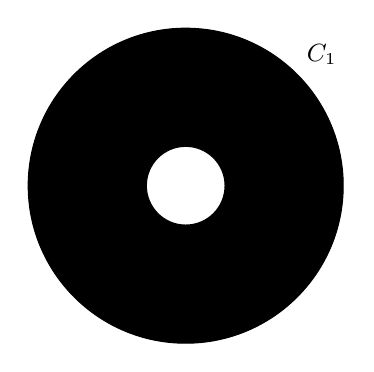
\begin{tikzpicture}
%  \usetikzlibrary{arrows}
  \filldraw [draw={\colorone},fill={\coloronefill}] (0,0) circle (2);
  \filldraw [draw={\colorone},fill=white] (0,0) circle (0.5);
  \node [above right] at (45:2) {\small $C_1$};
  \node [above] at (0,0.5) {\small $C_2$};
  \node at (0,1.35) {\small $R_1$};
  \node at (0,-1.35) {\small $R_2$};
  \node [rotate=45] at (135:.5) {$\blacktriangleright$};
  \node [rotate=45] at (-45:.5) {$\blacktriangleleft$};
  \node [rotate=-45] at (45:2) {$\blacktriangleleft$};
  \node [rotate=-45] at (-135:2) {$\blacktriangleright$};
  \draw [dashed] (0.5,0) --node[above]{$\to$}node[below]{$\leftarrow$} (2,0);
  \draw [dashed] (-0.5,0) --node[above]{$\to$}node[below]{$\leftarrow$} (-2,0);
 \end{tikzpicture}
 &
 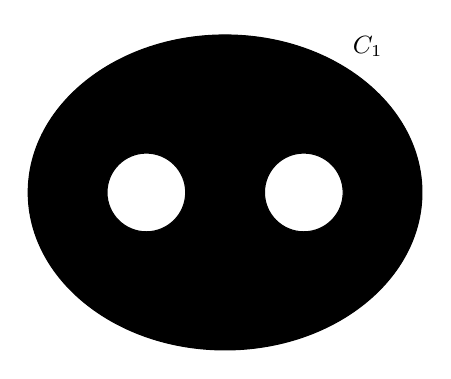
\begin{tikzpicture}
%  \usetikzlibrary{arrows}
  \filldraw [draw={\colorone},fill={\coloronefill}] (0,0) ellipse (2.5 and 2);
  \filldraw [draw={\colorone},fill=white] (-1,0) circle (0.5);
  \filldraw [draw={\colorone},fill=white] (1,0) circle (0.5);
  \node [above right] at (1.5,1.6) {\small $C_1$};
  \node [above] at (1,0.5) {\small $C_2$};
  \node [above] at (-1,0.5) {\small $C_3$};
  \node at (0,1.35) {\small $R_1$};
  \node at (0,-1.35) {\small $R_2$};
  \node [rotate=45] at (-1.3536,0.3536) {$\blacktriangleright$};
  \node [rotate=45] at (0.6464,0.3536) {$\blacktriangleright$};
  \node [rotate=45] at (-0.6464,-0.3536) {$\blacktriangleleft$};
  \node [rotate=45] at (1.3536,-0.3536) {$\blacktriangleleft$};
  \node [rotate=-31] at (1.5,1.6) {$\blacktriangleleft$};
  \node [rotate=-31] at (-1.5,-1.6) {$\blacktriangleright$};
  \draw [dashed] (2.5,0) --node[above]{$\to$}node[below]{$\leftarrow$} (1.5,0);
  \draw [dashed] (0.5,0) --node[above]{$\to$}node[below]{$\leftarrow$} (-0.5,0);
  \draw [dashed] (-1.5,0) --node[above]{$\to$}node[below]{$\leftarrow$} (-2.5,0);
 \end{tikzpicture} \\
 Region $R$ with one hole & Region $R$ with two holes
 \end{tabular}
 \caption{Multiply connected regions}
 \label{fig:multconn}
\end{lxfigure}

The intuitive idea for why Green's Theorem holds for multiply connected regions is shown in \autoref{fig:multconn} above. The idea is to cut ``slits'' between the boundaries of a multiply connected region $R$ so that $R$ is divided into subregions which do \emph{not} have any ``holes''. For example, in \autoref{fig:multconn}(a) the region $R$ is the union of the regions $R_1$ and $R_2$, which are divided by the slits indicated by the dashed lines. Those slits are part of the boundary of both $R_1$ and $R_2$, and we traverse then in the manner indicated by the arrows. Notice that along each slit the boundary of $R_1$ is traversed in the opposite direction as that of $R_2$, which means that the line integrals of \vecf\ along those slits add to 0. Since $R_1$ and $R_2$ do not have holes in them, then Green's Theorem holds in each subregion, so that
\[
 \oint_{\substack{\text{bdy}\\\text{of }R_1}}\vecf\cdot d\vecr = \iint_{R_1}
  \left( \frac{\partial Q}{\partial x} - \frac{\partial P}{\partial y} \right)\,dA \quad\text{and}\quad
 \oint_{\substack{\text{bdy}\\\text{of }R_2}}\vecf\cdot d\vecr = \iint_{R_2}
  \left( \frac{\partial Q}{\partial x} - \frac{\partial P}{\partial y} \right)\,dA .
\]
But since the line integrals along the slits are opposite each other, we have
\[
 \oint_{C_1 \cup C_2}\vecf\cdot d\vecr =
 \oint_{\substack{\text{bdy}\\\text{of }R_1}}\vecf\cdot d\vecr +
 \oint_{\substack{\text{bdy}\\\text{of }R_2}}\vecf\cdot d\vecr ,
\]
and so
\[
 \oint_{C_1 \cup C_2}\vecf\cdot d\vecr = \iint_{R_1}
  \left( \frac{\partial Q}{\partial x} - \frac{\partial P}{\partial y} \right)\,dA + \iint_{R_2}
  \left( \frac{\partial Q}{\partial x} - \frac{\partial P}{\partial y} \right)\,dA = \iint_{R}
  \left( \frac{\partial Q}{\partial x} - \frac{\partial P}{\partial y} \right)\,dA ,
\]
which shows that Green's Theorem holds in the region $R$. A similar argument shows that the theorem holds in the region with two holes shown in \autoref{fig:multconn}(b).

We know from \autoref{cor:lineintsuffpath} that when a smooth vector field $\vecf(x,y) = P(x,y)\,\veci + Q(x,y)\,\vecj$ on a region $R$ (whose boundary is a piecewise smooth, simple closed curve $C$) has a potential in $R$, then $\oint_{C}\vecf\cdot d\vecr = 0$. And if the potential $F(x,y)$ is smooth in $R$, then $\frac{\partial F}{\partial x} = P$ and $\frac{\partial F}{\partial y} = Q$, and so we know that
\[
 \frac{\partial^2 F}{\partial y \,\partial x} = \frac{\partial^2 F}{\partial x \,\partial y} \Rightarrow
 \frac{\partial P}{\partial y} = \frac{\partial Q}{\partial x} \text{ in $R$.}
\]
Conversely, if $\frac{\partial P}{\partial y} = \frac{\partial Q}{\partial x}$ in $R$ then
\[
 \oint_{C}\vecf\cdot d\vecr = \iint_{R} \left( \frac{\partial Q}{\partial x} -
   \frac{\partial P}{\partial y} \right)\,dA = \iint_{R} 0\,dA = 0 .
\]
For a \textbf{simply connected}\index{simply connected} region $R$ (i.e. a region with no holes), the following can be shown:\index{path independence}

\theorem{thm_equiv_path_indep}{Equivalence of Path Independence}{The following statements are equivalent for a simply connected region $R$ in $\mathbb{R}^2$:
  \begin{enumerate}
  \item $\vecf(x,y) = P(x,y)\,\veci + Q(x,y)\,\vecj$ has a smooth potential $F(x,y)$ in $R$
  \item $\ds{\int_{C}\vecf\cdot d\vecr}$ is independent of the path for any curve $C$ in $R$
  \item $\ds{\oint_{C}\vecf\cdot d\vecr} = 0$ for every simple closed curve $C$ in $R$
  \item $\dfrac{\partial P}{\partial y} = \dfrac{\partial Q}{\partial x}$ in $R$\quad
   (in this case, the differential form $P\,dx + Q\,dy$ is exact)\index{exact differential form}
 \end{enumerate}}

\printexercises{exercises/14_Greens_exercises}
